\newpage
\section{Open-loop System}

\subsection{System Model}

The chemical process illustrated in Figure~\ref{fig:reactor_scheme} represents an axial dispersion tubular reactor, which incorporates diffusion, convection, and a first-order irreversible chemical reaction \autocite{levenspiel1998chemical}. The reactor is equipped with a recycle mechanism, allowing a fraction of the product stream to re-enter the reactor to ensure the consumption of any unreacted substrate. By applying first-principle modeling through relevant mass balance relations on an infinitesimally small section of the reactor, the reactor's dynamics can be described by a second-order parabolic PDE, a common class of equations used to characterize diffusion-convection-reaction systems \autocite{jensen1982bifurcation}. The resulting PDE that describes the reactor model is given by:

\begin{equation} \label{eq:PDE_original_model}
    \dot{x}(\zeta, t) = D \partial_{\zeta \zeta} c(\zeta, t) - v \partial_\zeta c(\zeta, t) + k_r c(\zeta, t)
\end{equation}

subject to Dankwerts boundary conditions:

\begin{align} \label{eq:BC}
    \begin{cases}
        &D \partial_\zeta c(0, t) - v c(0, t) = -v \left[ R c(1, t-\tau) + (1-R) u(t) \right] \\
        &\partial_\zeta c(1, t) = 0 \\
        &y(t) = c(1, t)
    \end{cases}
\end{align}

Here, $c(\zeta, t)$ denotes the concentration along the reactor, representing the state of the system. The physical parameters $D$, $v$, $k_r$, $R$, and $\tau$ correspond to the diffusion coefficient, flow velocity along the reactor, reaction constant, recycle ratio, and residence time of the recycle stream, respectively. The spatial and temporal coordinates of the system are represented by $\zeta$ and $t$, where $\zeta \in [0, 1]$ and $t \in [0, \infty)$.

Dankwerts boundary conditions are particularly suitable for modeling axial tubular reactors, as they account for deviations from perfect mixing and piston flow, assuming negligible transport lags in connecting lines \autocite{danckwerts1993continuous}. These conditions make the model more realistic for chemical reactors of this type. The input and the output of the system are also present in the boundary conditions. The system output is measured at the reactor outlet, while the input is applied at the inlet. Additionally, the delayed state resulting from the recycled portion of the flow, occurring $\tau$ time units ago, is incorporated into the inlet; all as shown in Equation~\ref{eq:BC}.


\begin{figure}[ht]
    \centering
    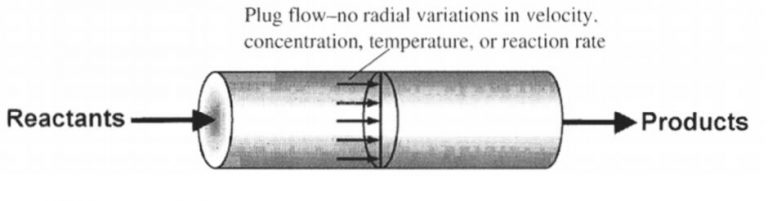
\includegraphics[width=0.7\textwidth]{Figures/sample.jpeg}
    \caption{Sample figure.}
    \label{fig:reactor_scheme}
\end{figure}

\subsection{PDE Representation of Delay Term}

One effective method for addressing delay in systems is to represent the delay using an alternative transport partial differential equation (PDE). This approach is particularly advantageous when the problem already involves similar forms of PDEs, as is the case in the current study. To specifically address the delay in the system under consideration, the state variable $c(\zeta, t)$ is expanded into a vector of functions $C(\zeta, t) \equiv [c_1(\zeta, t), c_2(\zeta, t)]^T$, where $c_1(\zeta, t)$ represents the concentration within the reactor, and $c_2(\zeta, t)$ is introduced as a new state variable to account for the concentration along the recycle stream. The delay is thus modeled as a pure transport process, wherein the first state $c_1(\zeta, t)$ is transported from the reactor outlet to the inlet, experiencing a delay of $\tau$ time units while in the recycle stream. As a result, Equations~\ref{eq:PDE_original_model}~and~\ref{eq:BC} may be re-formulated as follows:

\begin{align}
    \partial_t 
    \begin{bmatrix}
        c_1(\zeta, t) \\ c_2(\zeta,t)
    \end{bmatrix}
    =
    \begin{bmatrix}
        D \partial_{\zeta \zeta} - v \partial_\zeta + k_r && 0 \\
        0 && -\frac{1}{\tau} \partial_\zeta
    \end{bmatrix}
    \begin{bmatrix}
        c_1(\zeta, t) \\ c_2(\zeta,t)
    \end{bmatrix}\\
\begin{cases}
    D \partial_\zeta c_1(0, t) - v c_1(0, t) = -v \left[ R c_2(0, t) + (1-R) u(t) \right] \\
    \partial_\zeta c_1(1, t) = 0 \\
    c_1(1,t) = c_2(1,t) \\
    y(t) = c_1(1, t)
\end{cases}
\end{align}

With all state variables now expressed explicitly at a specific time instance $t$—in contrast to the previous representation where states at $t$ were directly involved with states at $t-\tau$—the system can be described in the standard state-space form of an infinite-dimensional linear time-invariant (LTI) system as $\dot{x} = \mathfrak{A} x$. Here, the state $x(\zeta, t) = [x_1(\zeta, t), x_2(\zeta, t)]^T$ is a vector of functions, and $\mathfrak{A}$ is a linear operator $\mathcal{L}(X)$ acting on a Hilbert space $X: L^2[0,1] \times L^2[0,1]$. The operator $\mathfrak{A}$ and its domain are defined in detail as shown in Equation~\ref{eq:operator_A}:

\begin{equation} \label{eq:operator_A}
    \begin{aligned}
        \mathfrak{A} \equiv&
        \begin{bmatrix}
            D \partial_{\zeta \zeta} - v \partial_\zeta + k_r && 0 \\
            0 && -\frac{1}{\tau} \partial_\zeta
        \end{bmatrix}\\
        D(\mathfrak{A}) =& \{ x = [x_1, x_2]^T \in X:
        x(\zeta), \partial_\zeta x(\zeta), \partial_{\zeta \zeta} x(\zeta) \quad \mathrm{a.c.},\\
        &D \partial_\zeta x_1(0) - v x_1(0) = -v \left[ R x_2(0) + (1-R) u \right],\\
        &\partial_\zeta x_1(1) = 0,
        x_1(1) = x_2(1)\}
    \end{aligned}
\end{equation}

\subsection{Adjoint Operator}

\subsection{Choice of System Parameters}

\subsection{Eigenvalue Analysis}

\subsection{Eigenfunctions Representation}

\subsection{Open-loop (Zero-input) Response}